\chapter{Desigualdad social }
\section{Tipos de igualdad jurídica}
\subsection{Igualdad ante la ley}
\subsection{Igualdad mediante la ley}

\section{Igualdad, equidad y justícia }
 Figura \ref{fig:DesigualdadSocial}

\begin{figure}[ht!]
    \centering
    \begin{subfigure}{0.3\textwidth}
        \caption{Igualdad.}
        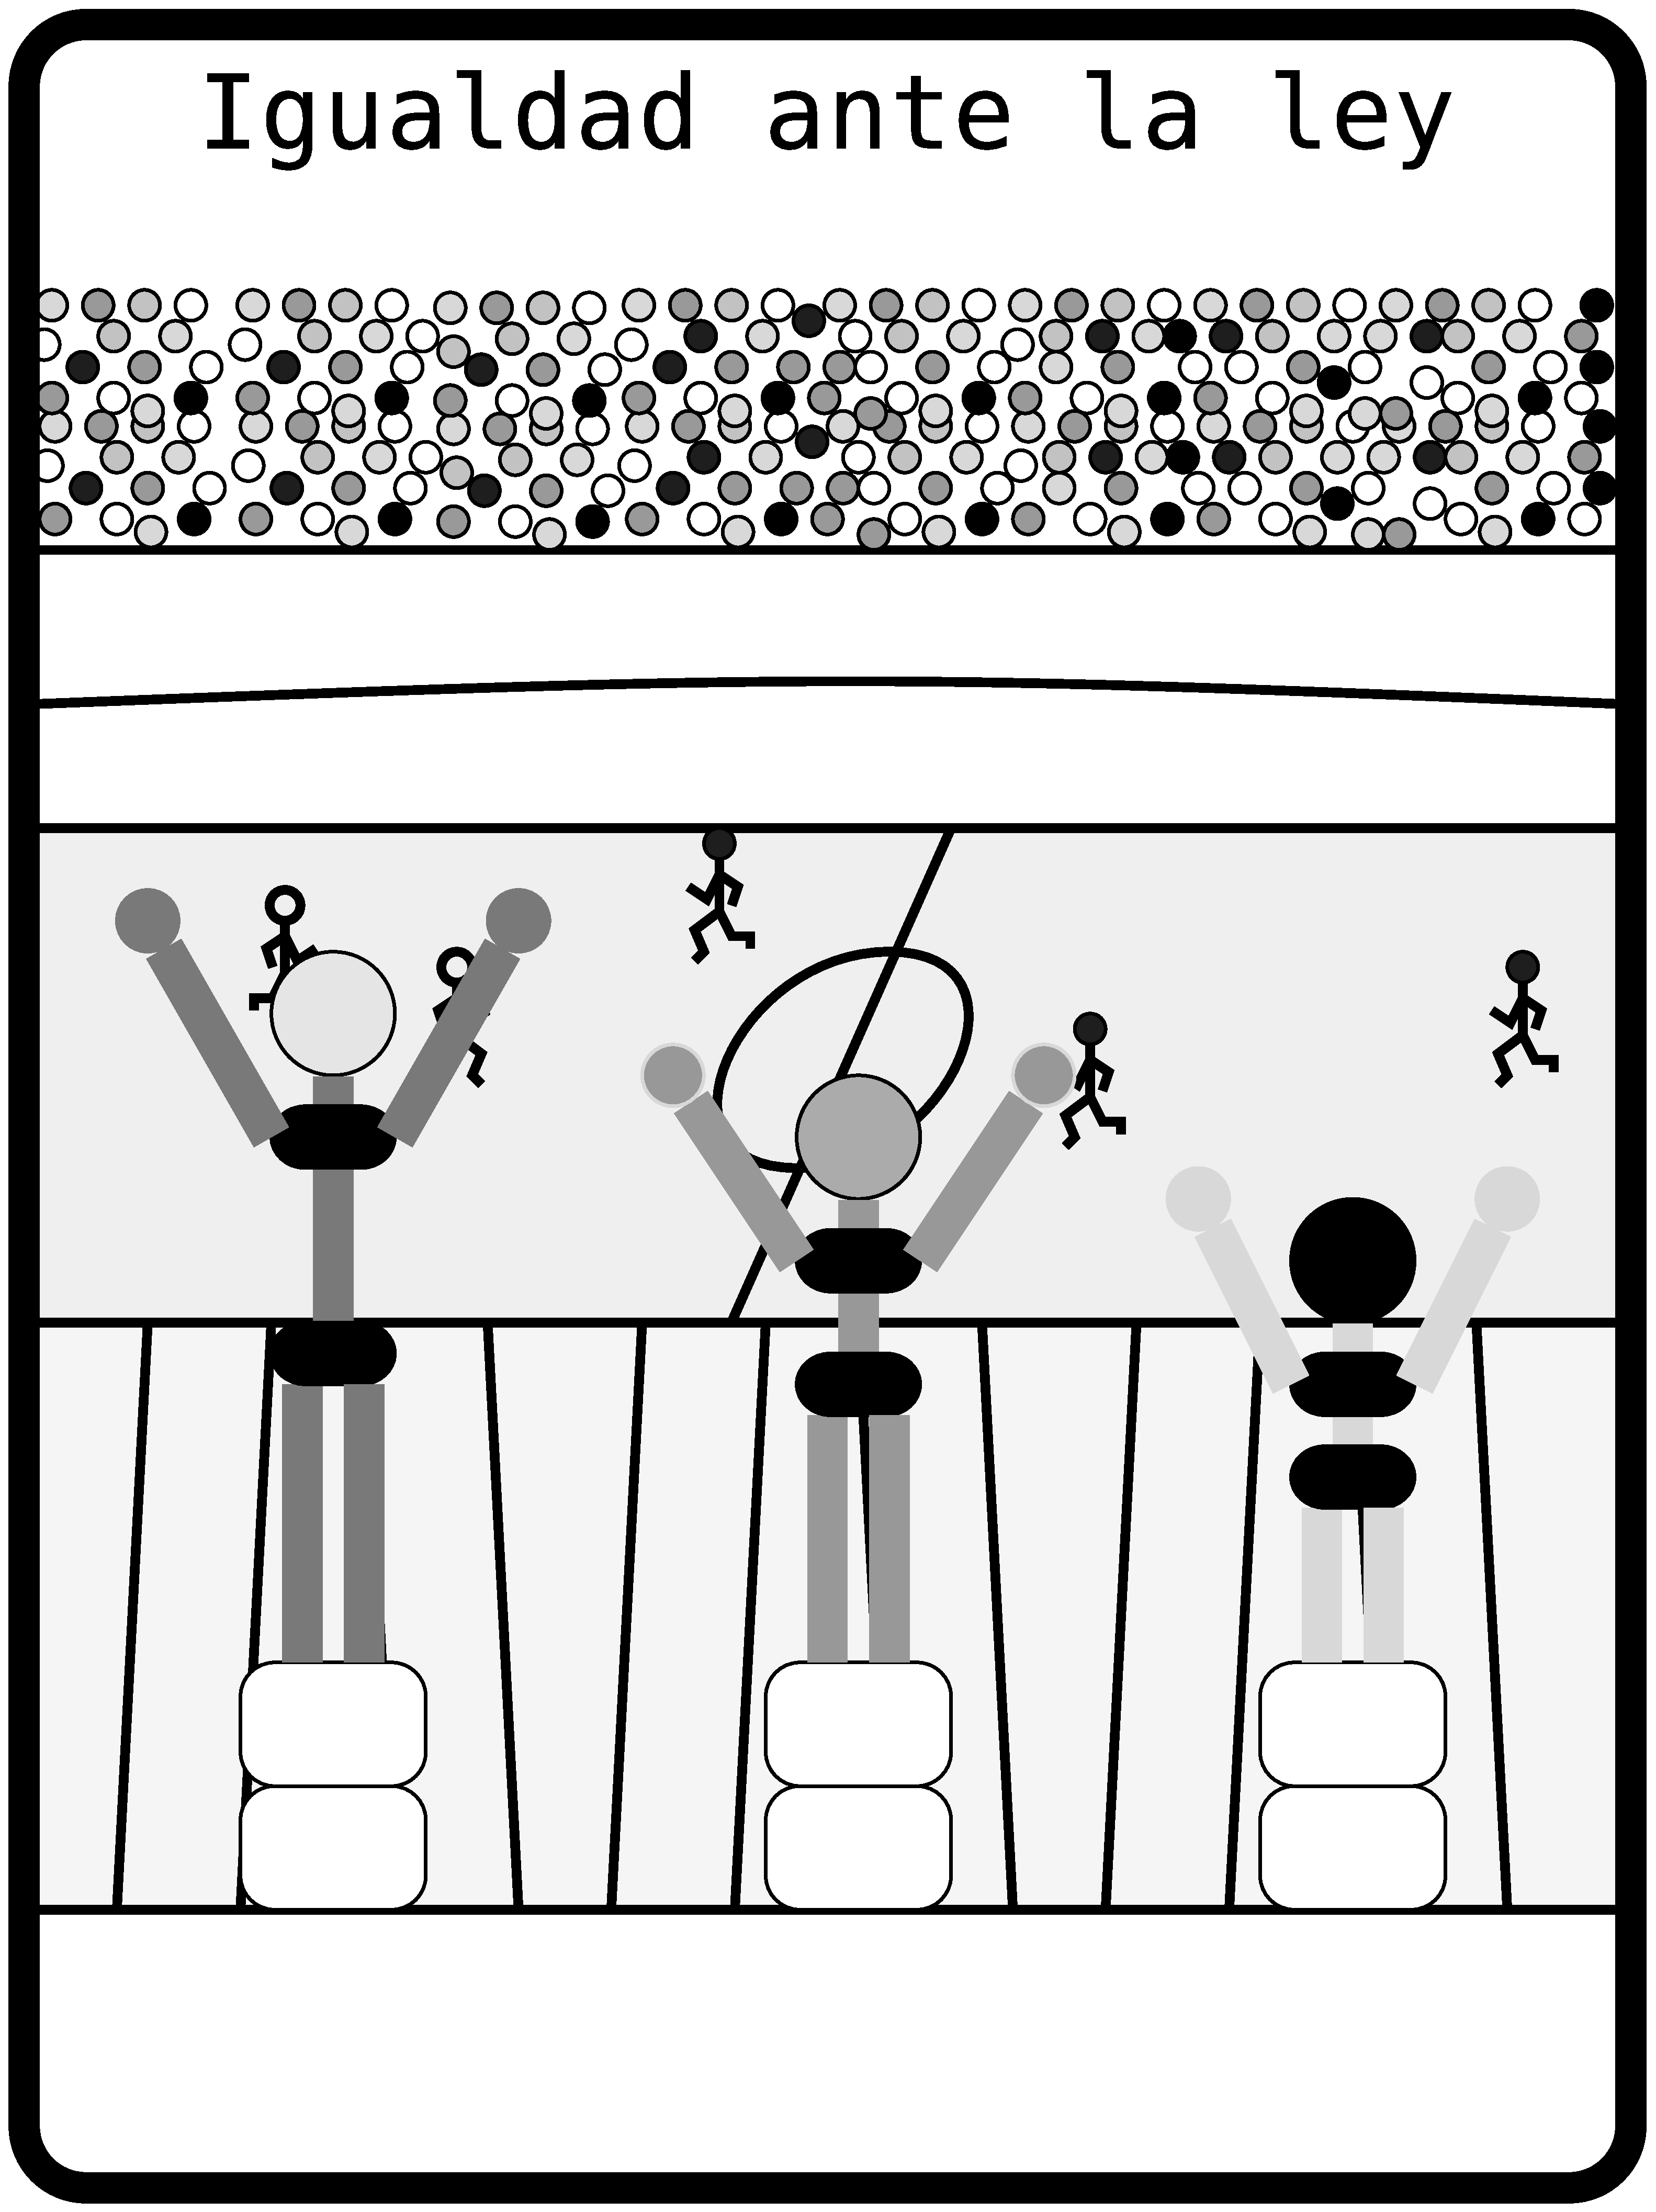
\includegraphics[width=\textwidth]{caps/desigualdad/igualdad.eps}
        \label{fig:igualdad}
    \end{subfigure}
    ~ %add desired spacing between images, e. g. ~, \quad, \qquad, \hfill etc. 
      %(or a blank line to force the subfigure onto a new line)
    \begin{subfigure}{0.3\textwidth}
        \caption{Equidad.}
        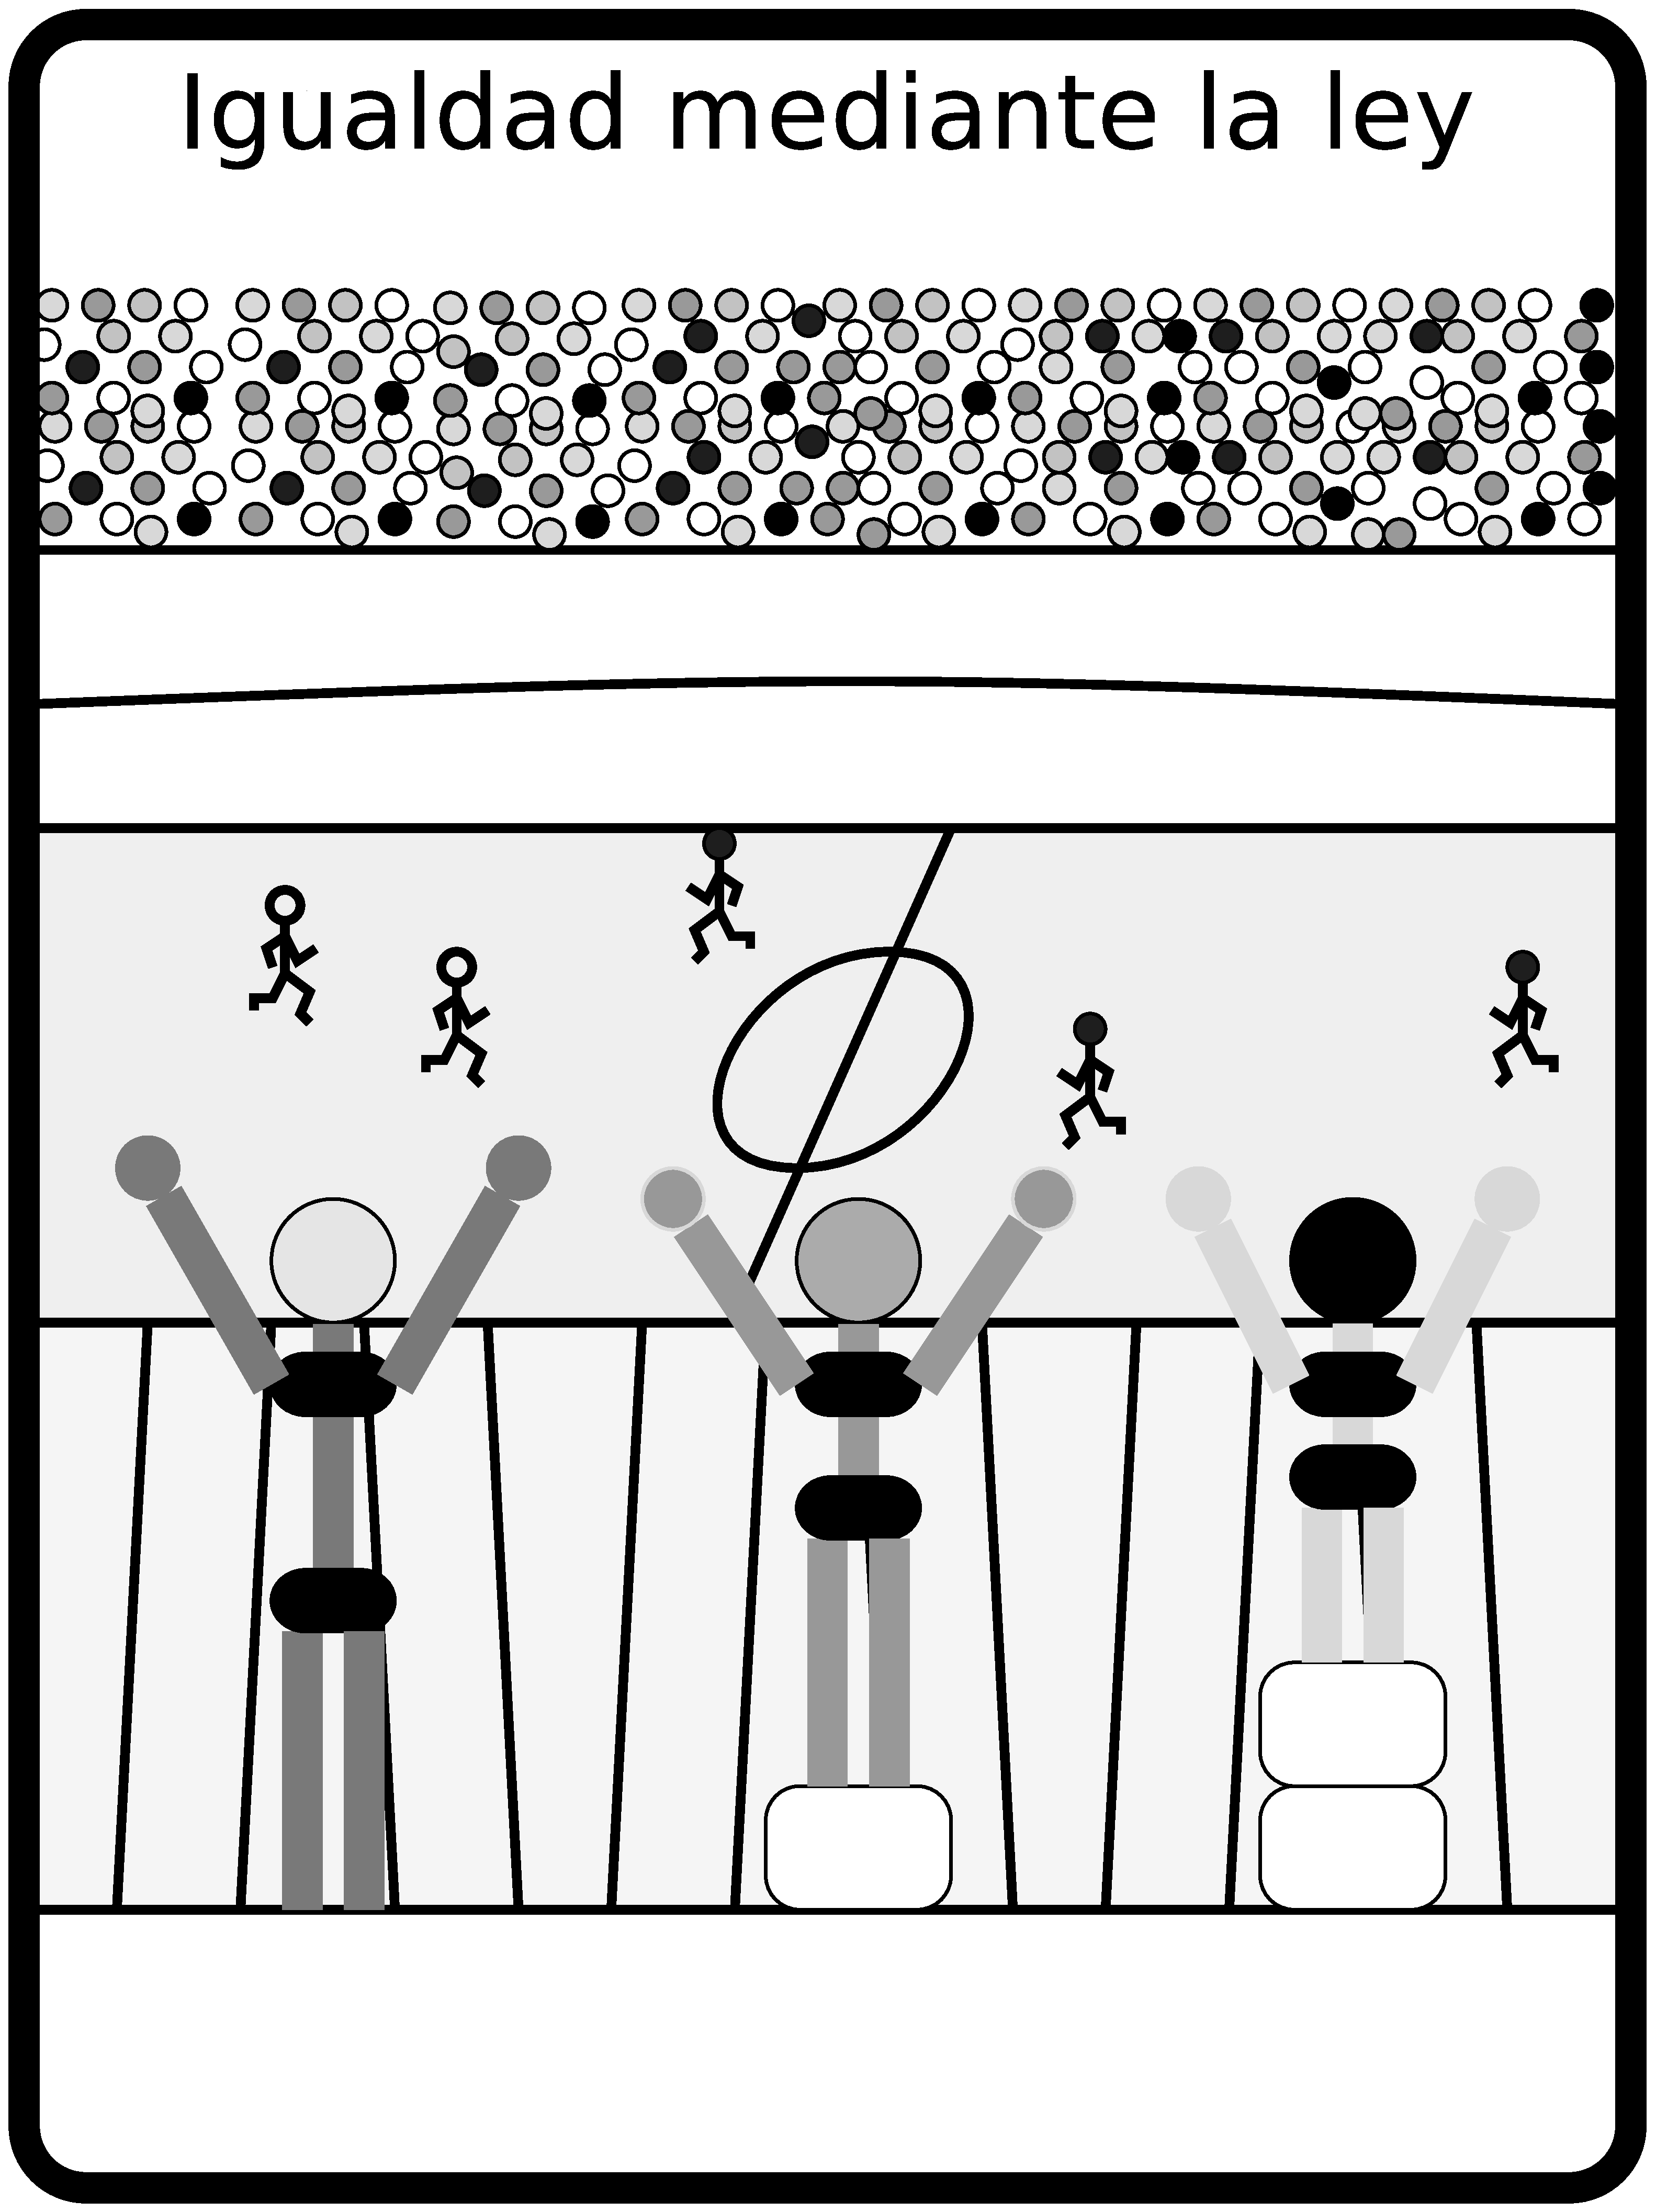
\includegraphics[width=\textwidth]{caps/desigualdad/equidad.eps}
        \label{fig:equidad}
    \end{subfigure}
    ~ %add desired spacing between images, e. g. ~, \quad, \qquad, \hfill etc. 
      %(or a blank line to force the subfigure onto a new line)
    \begin{subfigure}{0.3\textwidth}
        \caption{Justicia.}
        \includegraphics[width=\textwidth]{caps/desigualdad/justicia.eps}
        \label{fig:justicia}
    \end{subfigure}
    \caption{Desigualdad social.}\label{fig:DesigualdadSocial}
\end{figure}

\subsection{Igualdad}

El estado no genera riquesa, y tiene el trabajo de repartirla por igual a todos.
\subsection{Equidad}
El estado no genera riquesa, y tiene el trabajo de repartirla con equidad bajos su propia subjetividad.

Quien medirá la subjetividad de la desigualdad, con que criterio y con que autoridad.
\subsection{Justícia}
El estado no genera riquesa, Usa sus recursos pra crear un escenario que ayude a todos
independientemente de sus particularidades.
